\section{Interfaces de usuario}
A continuación se realiza la presentación del demo que se espera del producto final.
\subsection{App}

\subsubsection{Registrar nueva cuenta:}
A través de esta interfaz se puede registrar los datos básicos del usuario para poder utilizar la aplicación.

Los datos solicitados son:

\begin{itemize}[noitemsep]
\item Nombre
\item Apellido
\item Nombre de usuario: para el login
\item Email
\item Contraseña
\end{itemize}

Cuando se genera el registro, se crea un usuario en el sistema, pero solo estará activo hasta cuando active su cuenta por correo.

\begin{figure}[h!]
 \centering
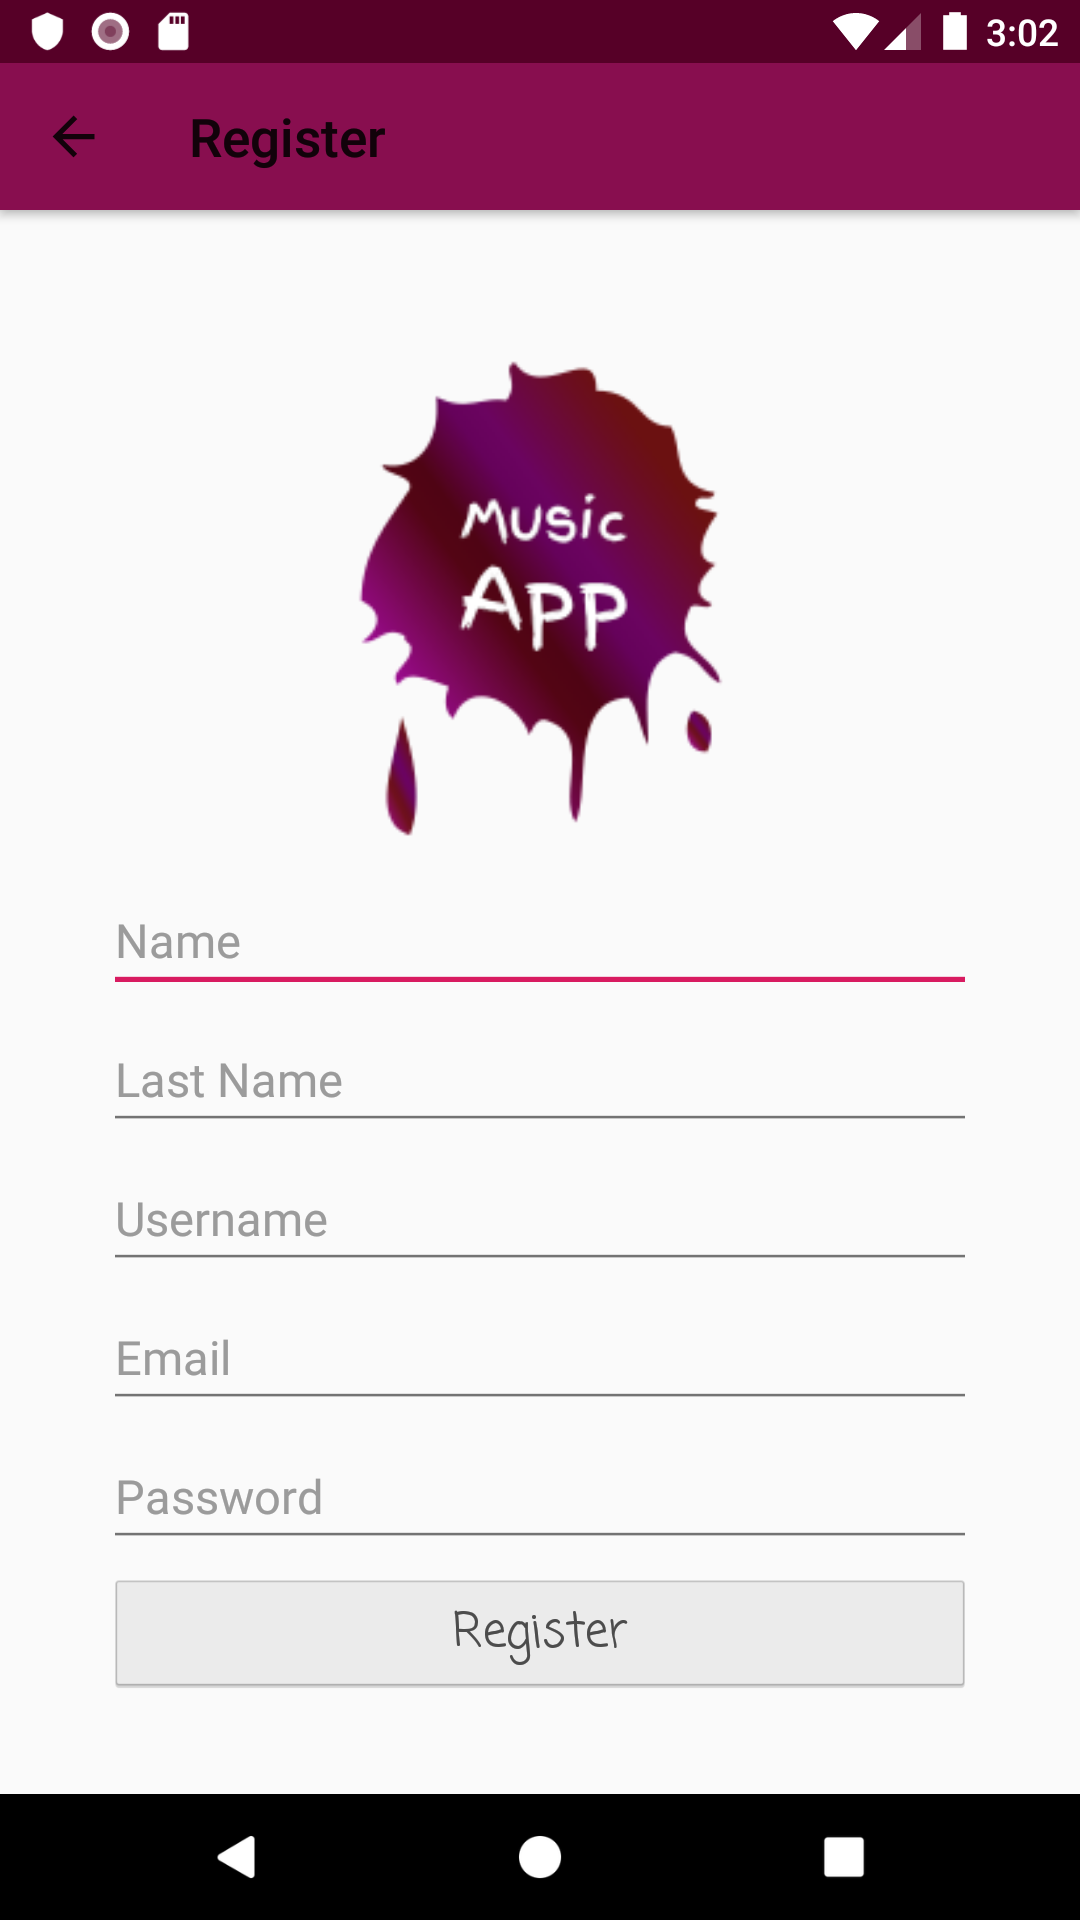
\includegraphics[width=0.6\linewidth]{Desarrollo/Interfaces/Interfaces/imgs/register.png}
\caption{Vista de registro de usuario en MusicApp}
\end{figure}

\newpage

\subsubsection{Correo de activación:}
Una vez hecho el registro en la app tiene que activar al cuenta para hacer uso de la misma.\\

Va a llegar un mensaje a la dirección de correo registrada, con un link que permitirá el acceso a la cuenta.\\

Una vez ingrese al link le debe aparecer una vista de activación como se muestra en la imagen \ref{fig:activation}\\


\begin{lstlisting}
Dear lautaro14

Your MusicApp account has been created, please click on the URL below to activate it:

http://misicapp.com/#/activate?key=28472109262983183349

Regards, 
Musicapp Team.
\end{lstlisting}

\begin{figure}[h!]
 \centering
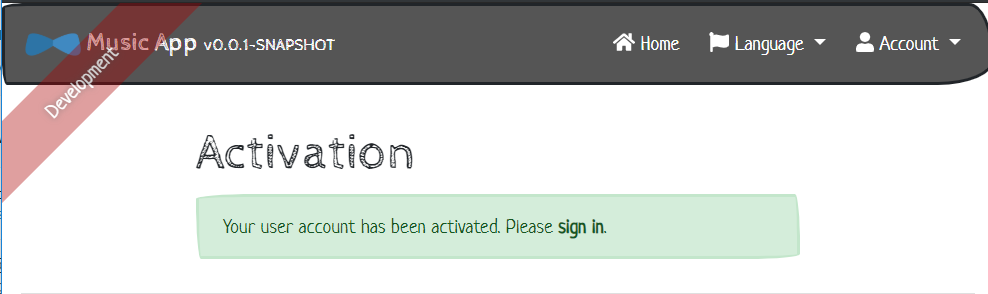
\includegraphics[width=\linewidth]{Desarrollo/Interfaces/Interfaces/imgs/activation.PNG}
\caption{Vista de una activación exitosa de la cuenta}
\label{fig:activation}
\end{figure}

\subsubsection{Iniciar Sesión:}
Una vez realizado el registro y la activación de la cuenta, se proceda a hacer el login. Se puede hacer con el email o con el nombre de usuario ingresado en el registro.
\begin{figure}[h!]
 \centering
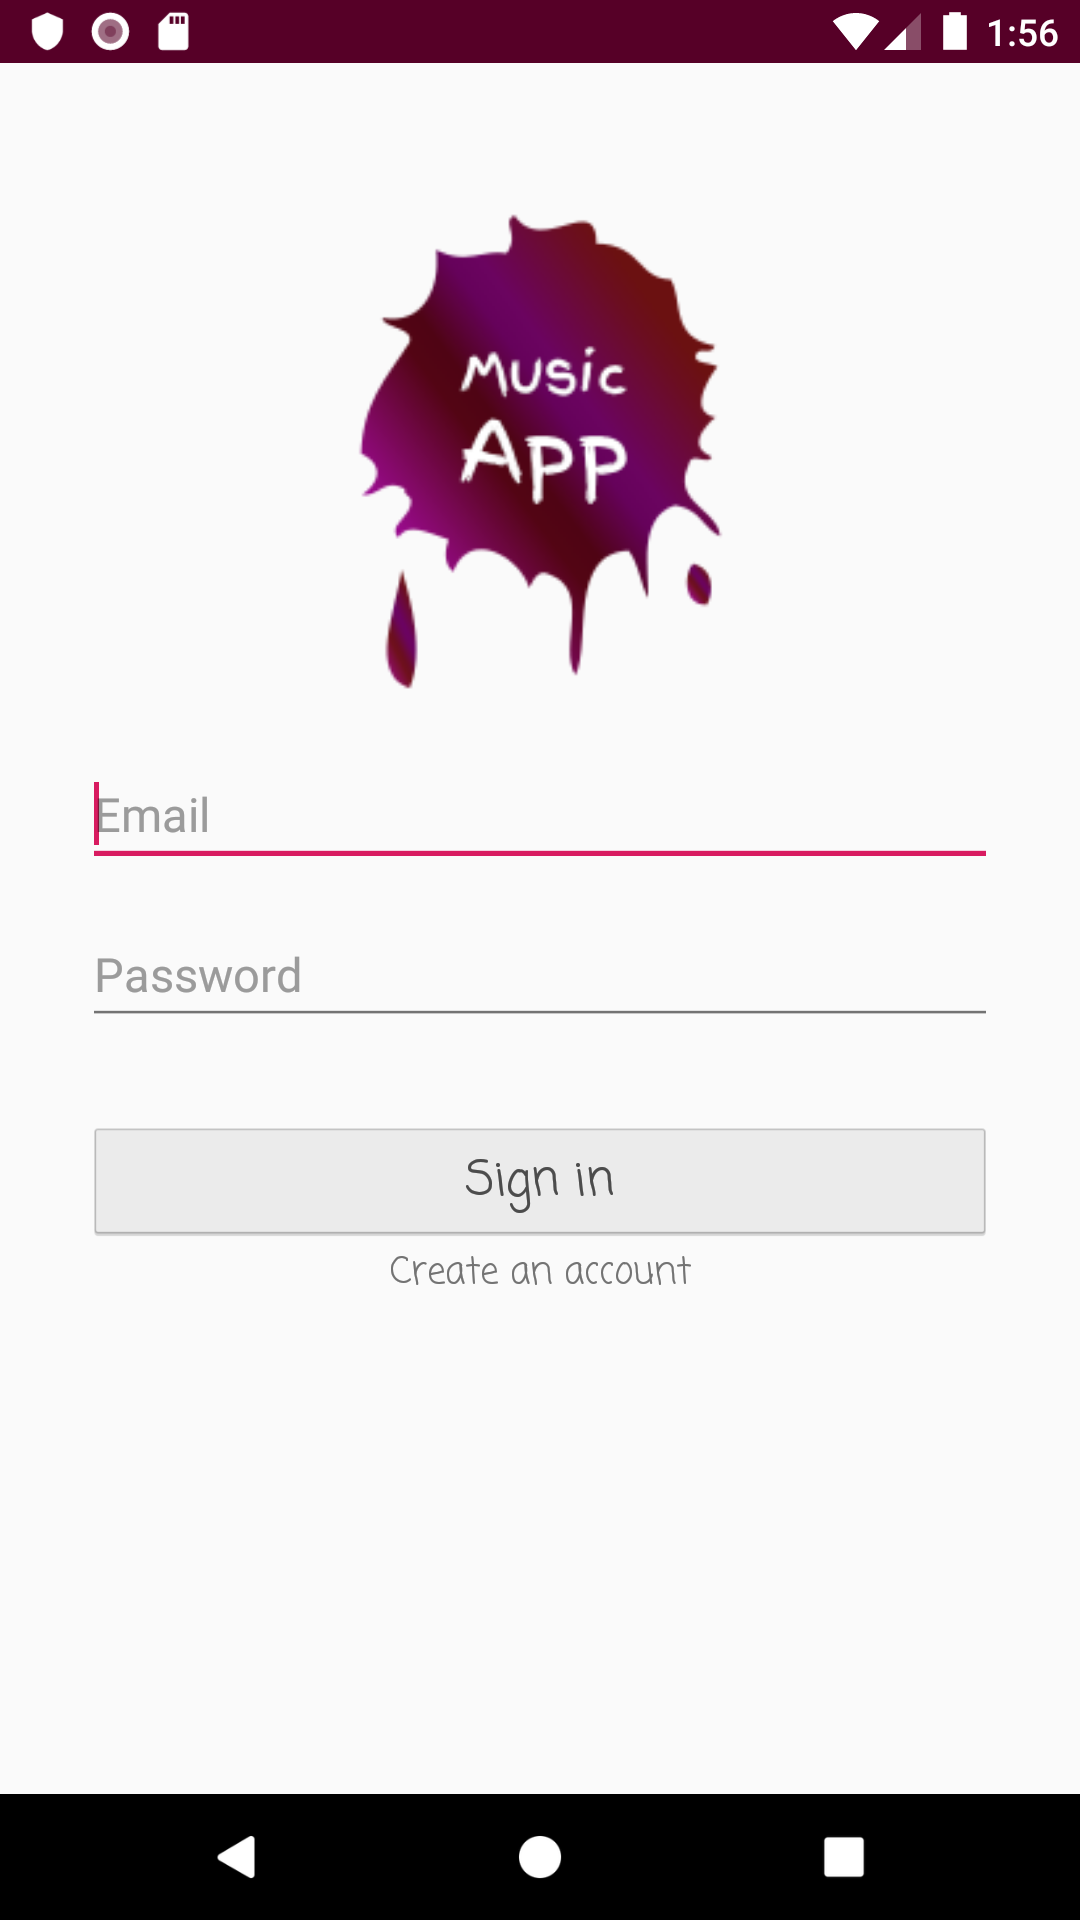
\includegraphics[width=0.6\linewidth]{Desarrollo/Interfaces/Interfaces/imgs/login.png}
\caption{Vista de login}
\end{figure}

\newpage

\subsubsection{Visualización ofertas:}

Apenas ingrese, se va a ver las lista de los músicos más destacados. \\

Se puede filtrar por nombre o por categoría del grupo musical. La información que se puede ver de los músicos es, una foto representativa, el nombre del grupo, su categoría y la calificación. \\


\begin{figure}[hbt!]
\centering
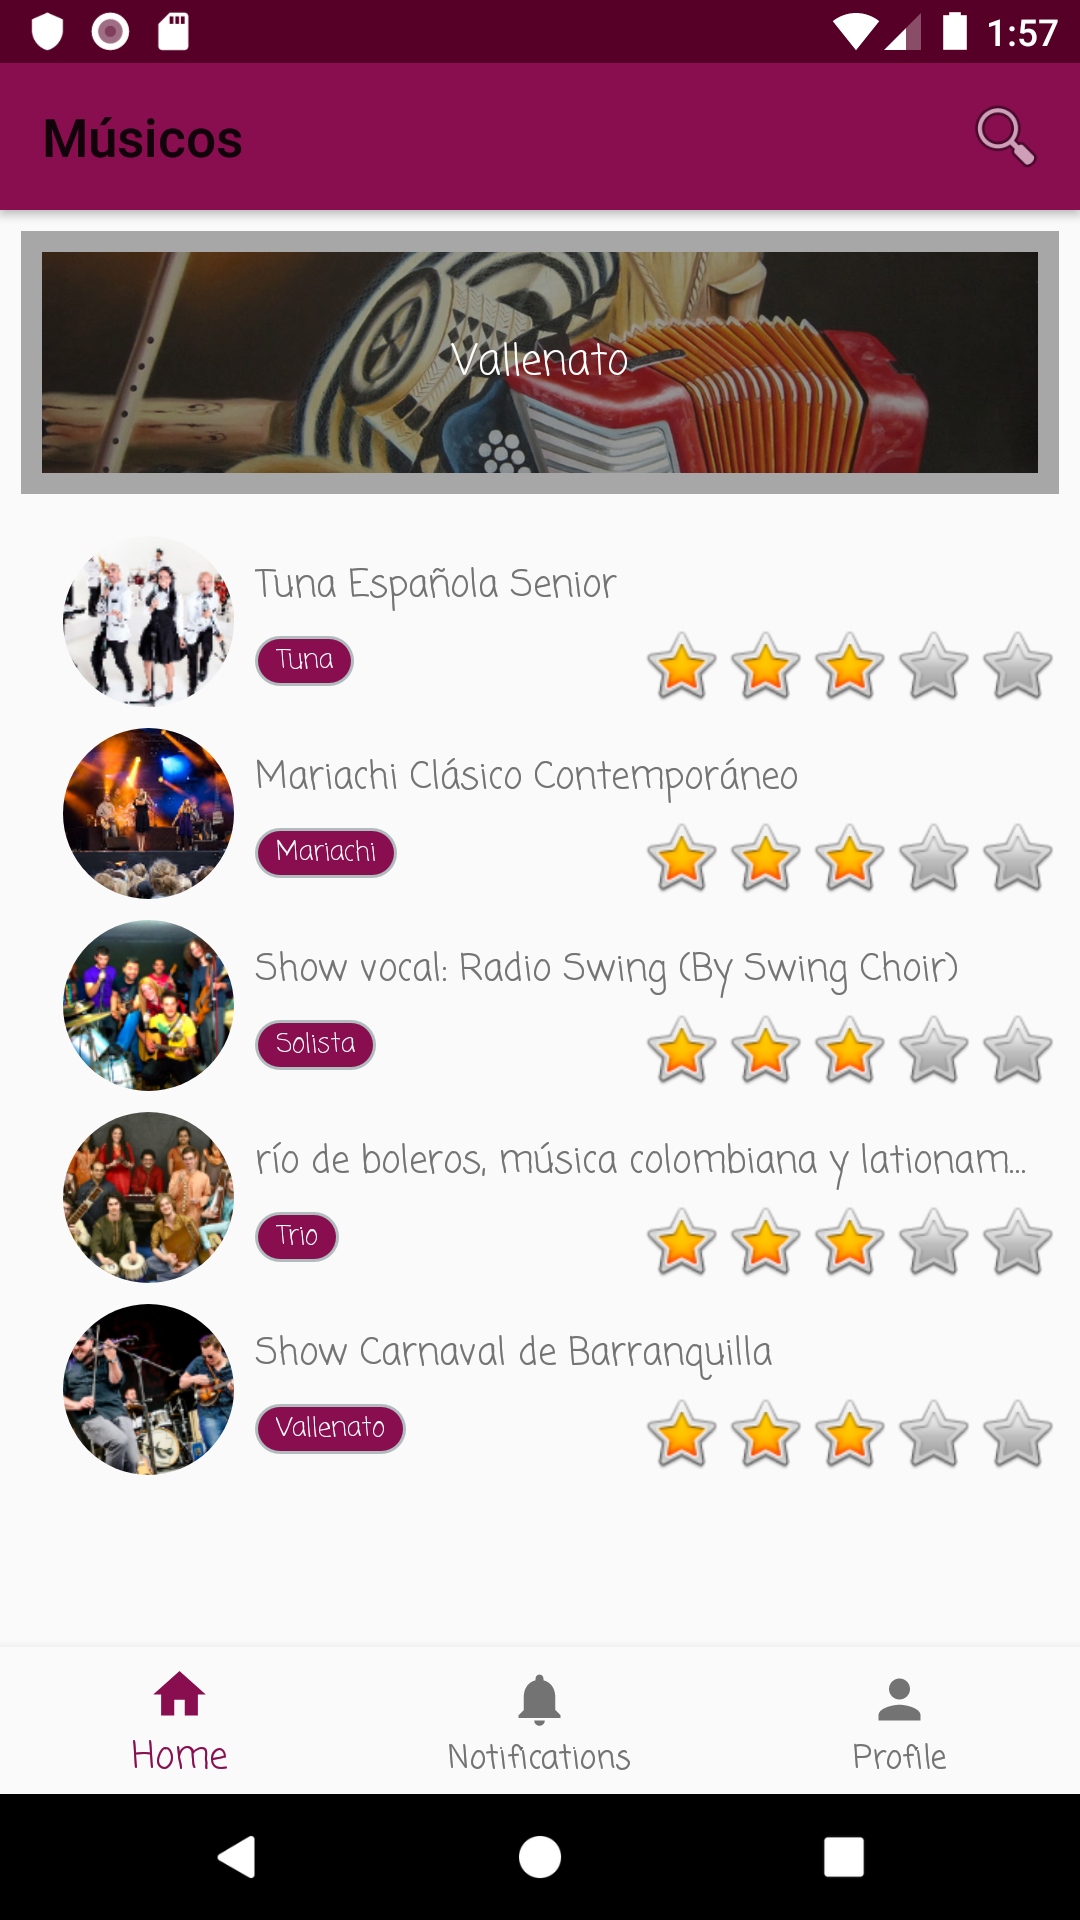
\includegraphics[width=0.6\linewidth]{Desarrollo/Interfaces/Interfaces/imgs/list.png}
\caption{Vista de oferta de músicos}
\end{figure}
\newpage
\subsubsection{Detalle Musico:}
Cuando se quiere tener más información de un  músico, se presenta en la siguiente vista. \\
Se puede ver el vídeo del artista, las fotos de eventos que hayan tenido, la calificación y una descripción corta de los servicios que ofrecen. 
\begin{figure}[hbt!]
 \centering
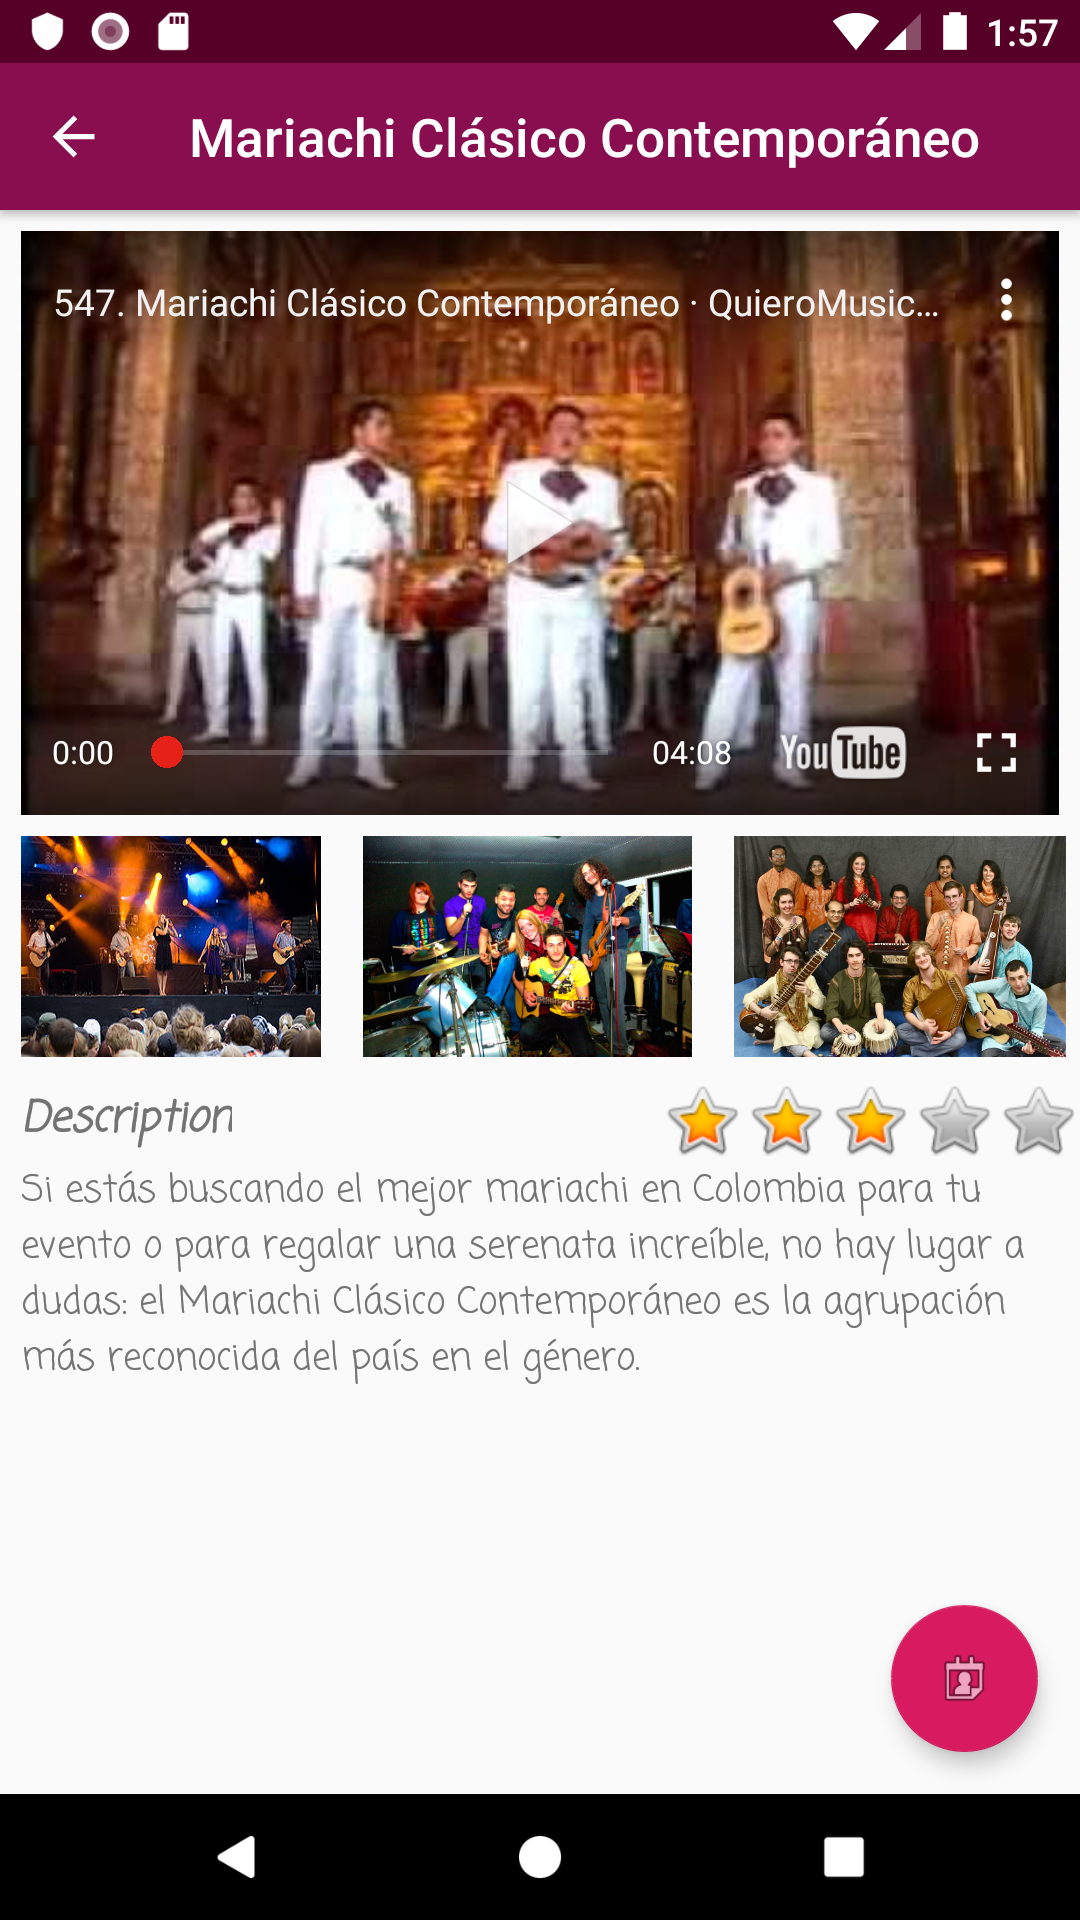
\includegraphics[width=0.6\linewidth]{Desarrollo/Interfaces/Interfaces/imgs/detail.png}
\caption{Vista de detalle del músico}
\end{figure}
\newpage

\subsubsection{Solicitud de servicios:}
Si se está interesado en un servicio de un músico, aquí se puede realizar una cotización, indicando los datos de contacto, la dirección la fecha e información adicional. 
\begin{figure}[hbt!]
 \centering
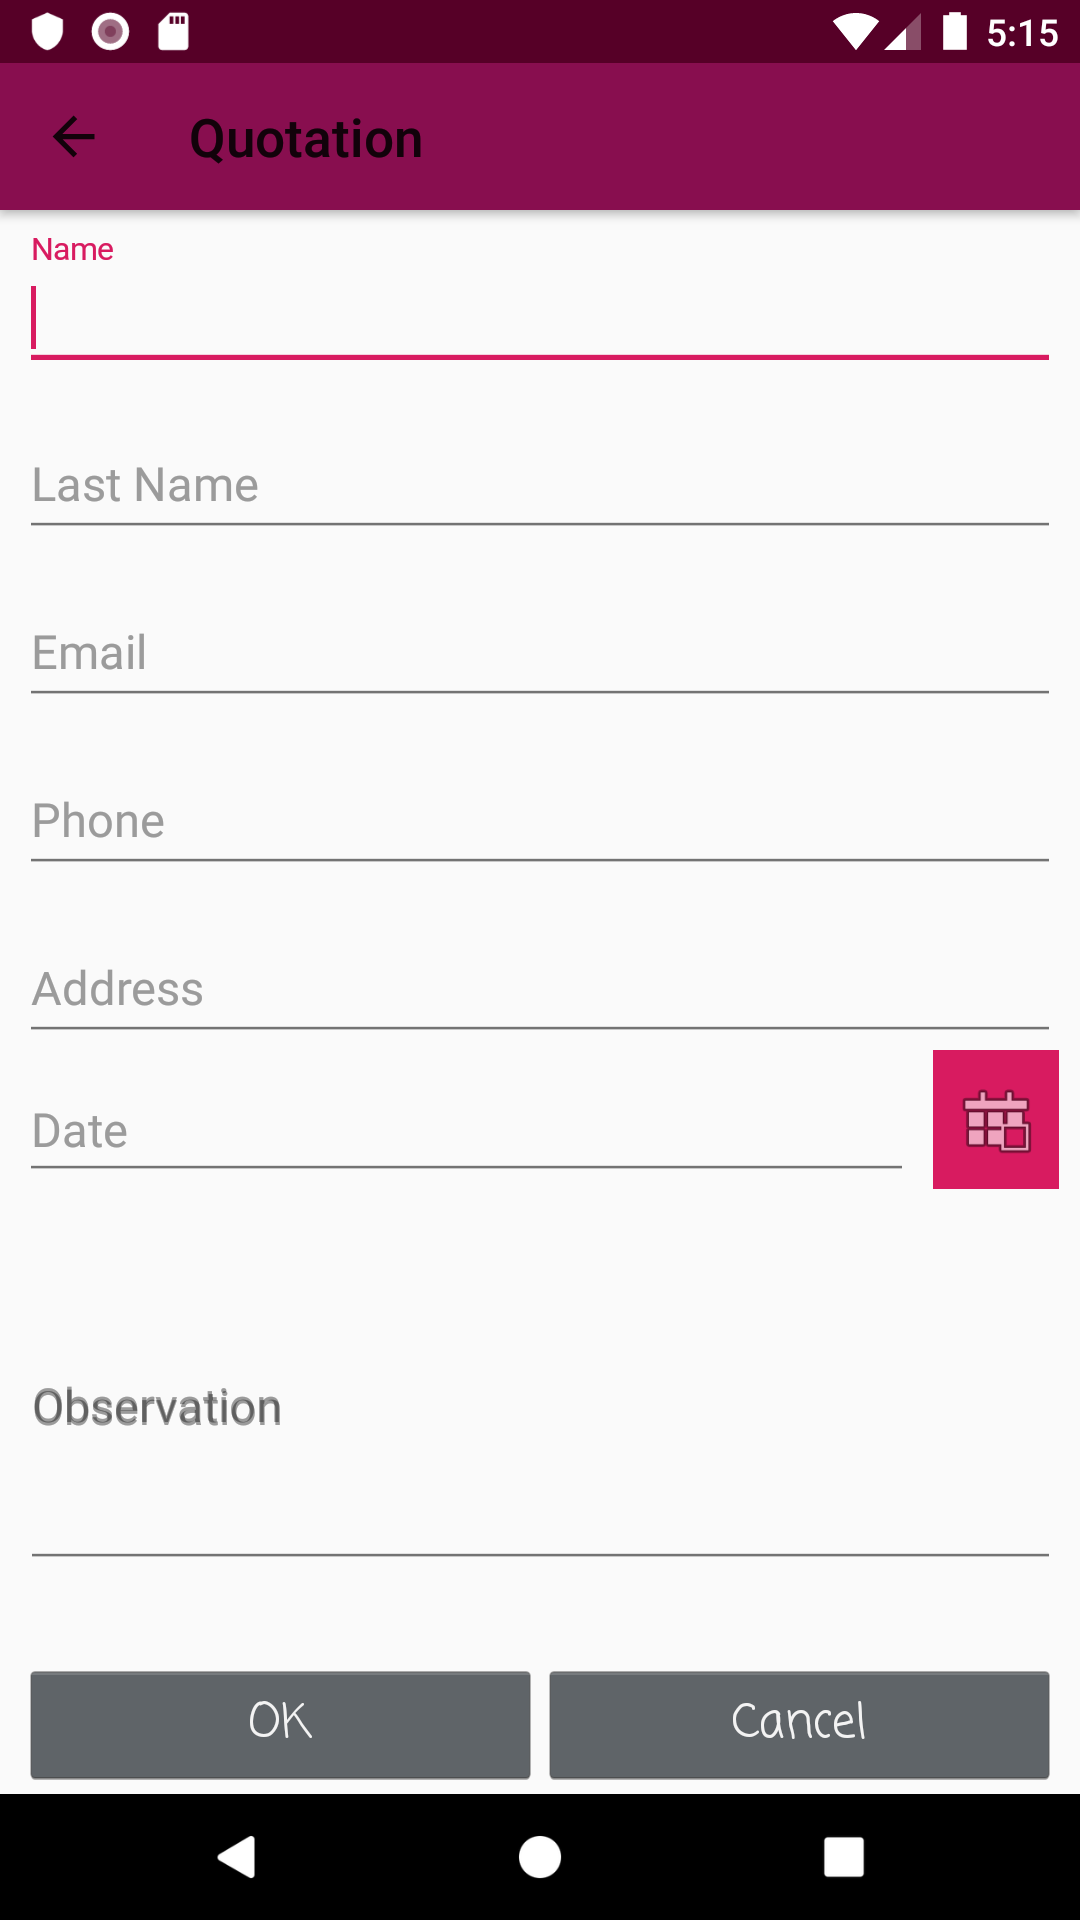
\includegraphics[width=0.6\linewidth]{Desarrollo/Interfaces/Interfaces/imgs/quotation.png}
\caption{Solicitar cotización}
\end{figure}

\newpage

\subsubsection{Cotizaciones realizadas y perfil:}
En esta vista puede ver los datos básicos del usuario, y la información de las reservas que ha hecho.
\begin{figure}[hbt!]
 \centering
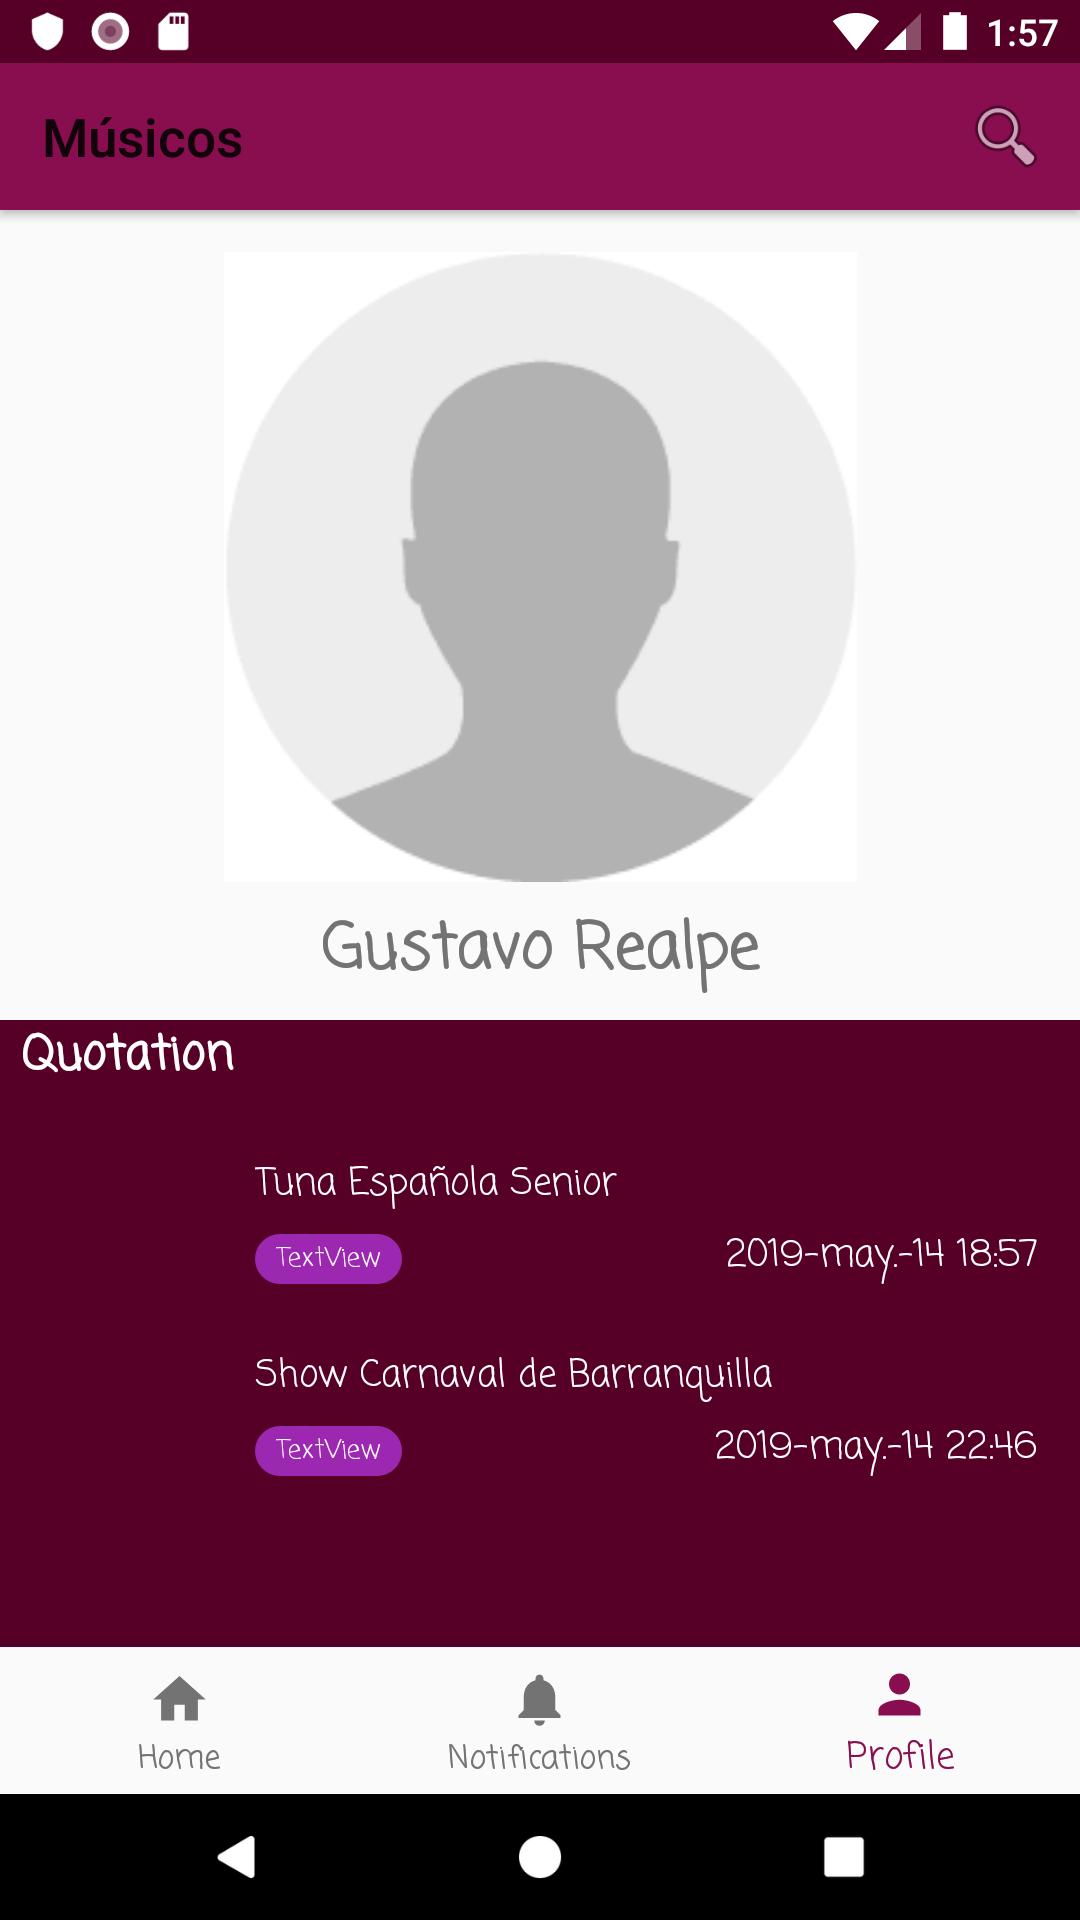
\includegraphics[width=0.6\linewidth]{Desarrollo/Interfaces/Interfaces/imgs/profile.png}
\caption{Vista de perfil y cotizaciones realizadas}
\end{figure}
\newpage


\subsection{Administración}
En la siguiente sección, se muestran las vistas del módulo de administración de MusicApp, es una aplicación desarrollada en Angular, es web y se pueden administrar valores y parámetros de la aplicación.
\subsubsection{Listar Grupos musicales}
En esta vista podemos ver y organizar los grupos musicales que han sido registrados en el sistema.
\begin{figure}[h!]
 \centering
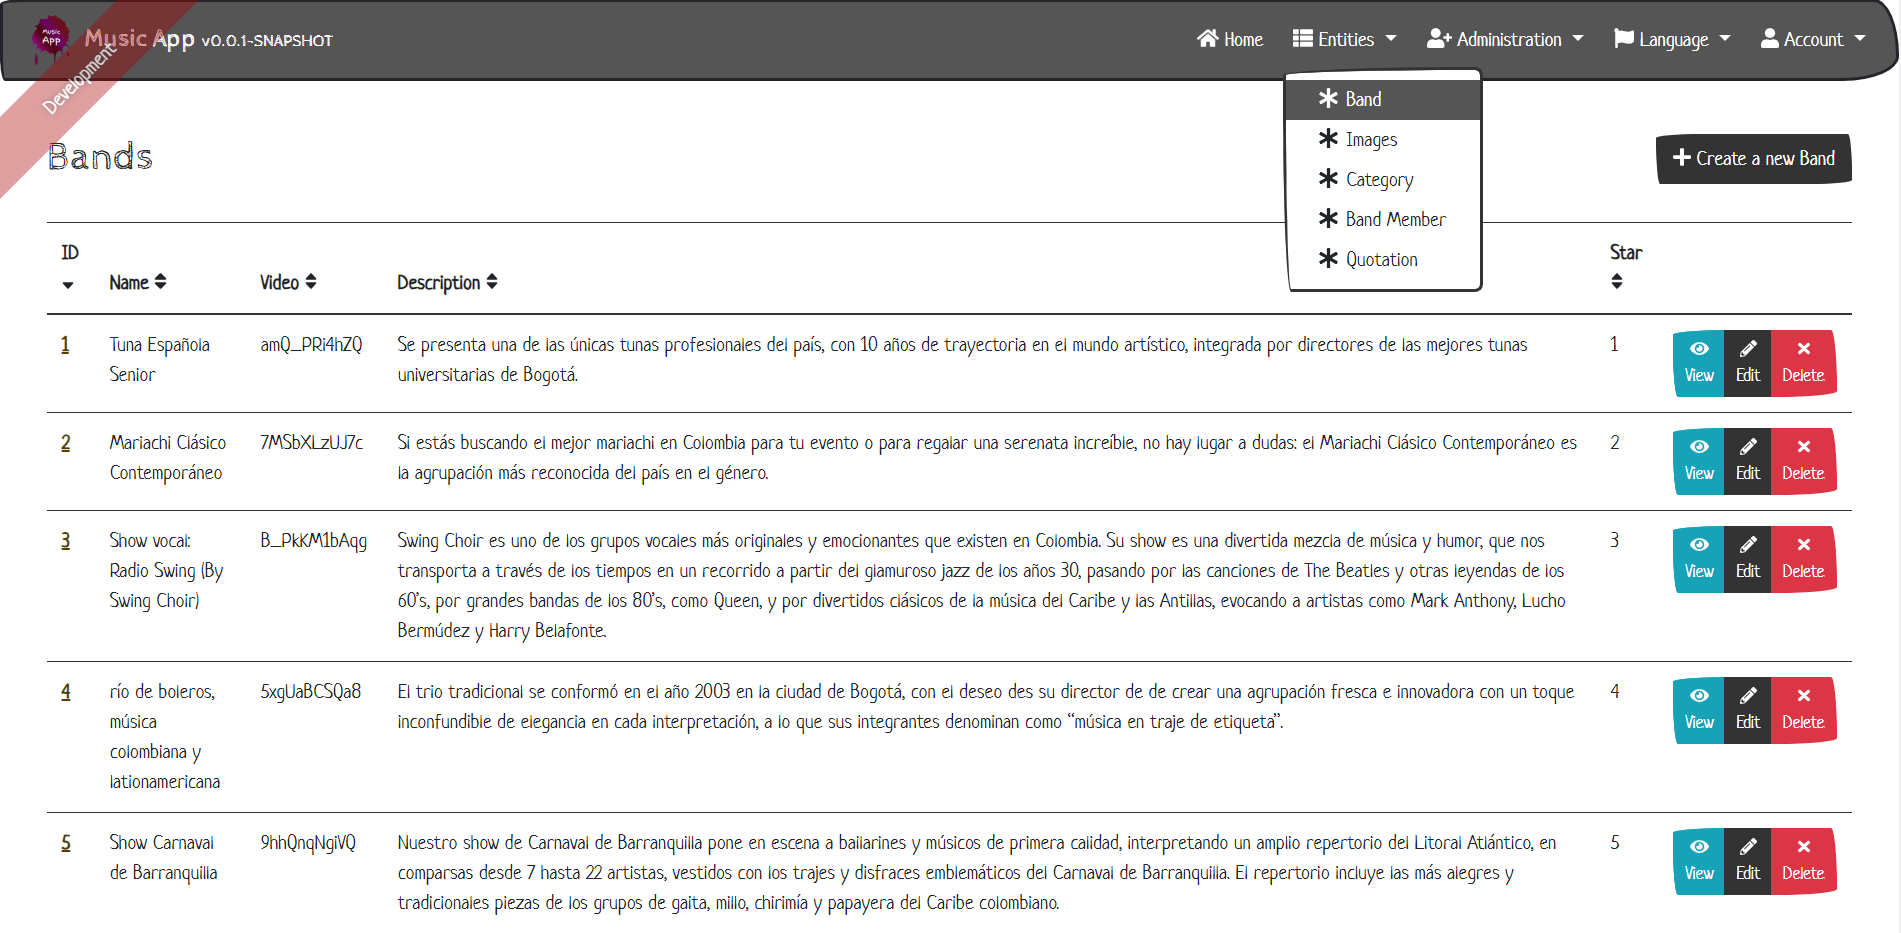
\includegraphics[width=\linewidth]{Desarrollo/Interfaces/Interfaces/imgs/BandList.PNG}
\caption{Lista de grupos musicales}
\end{figure}

\newpage

\subsubsection{Editar o crear Grupos musicales}
En esta vista podemos editar la información de un grupo musical en especial.
\begin{figure}[h!]
 \centering
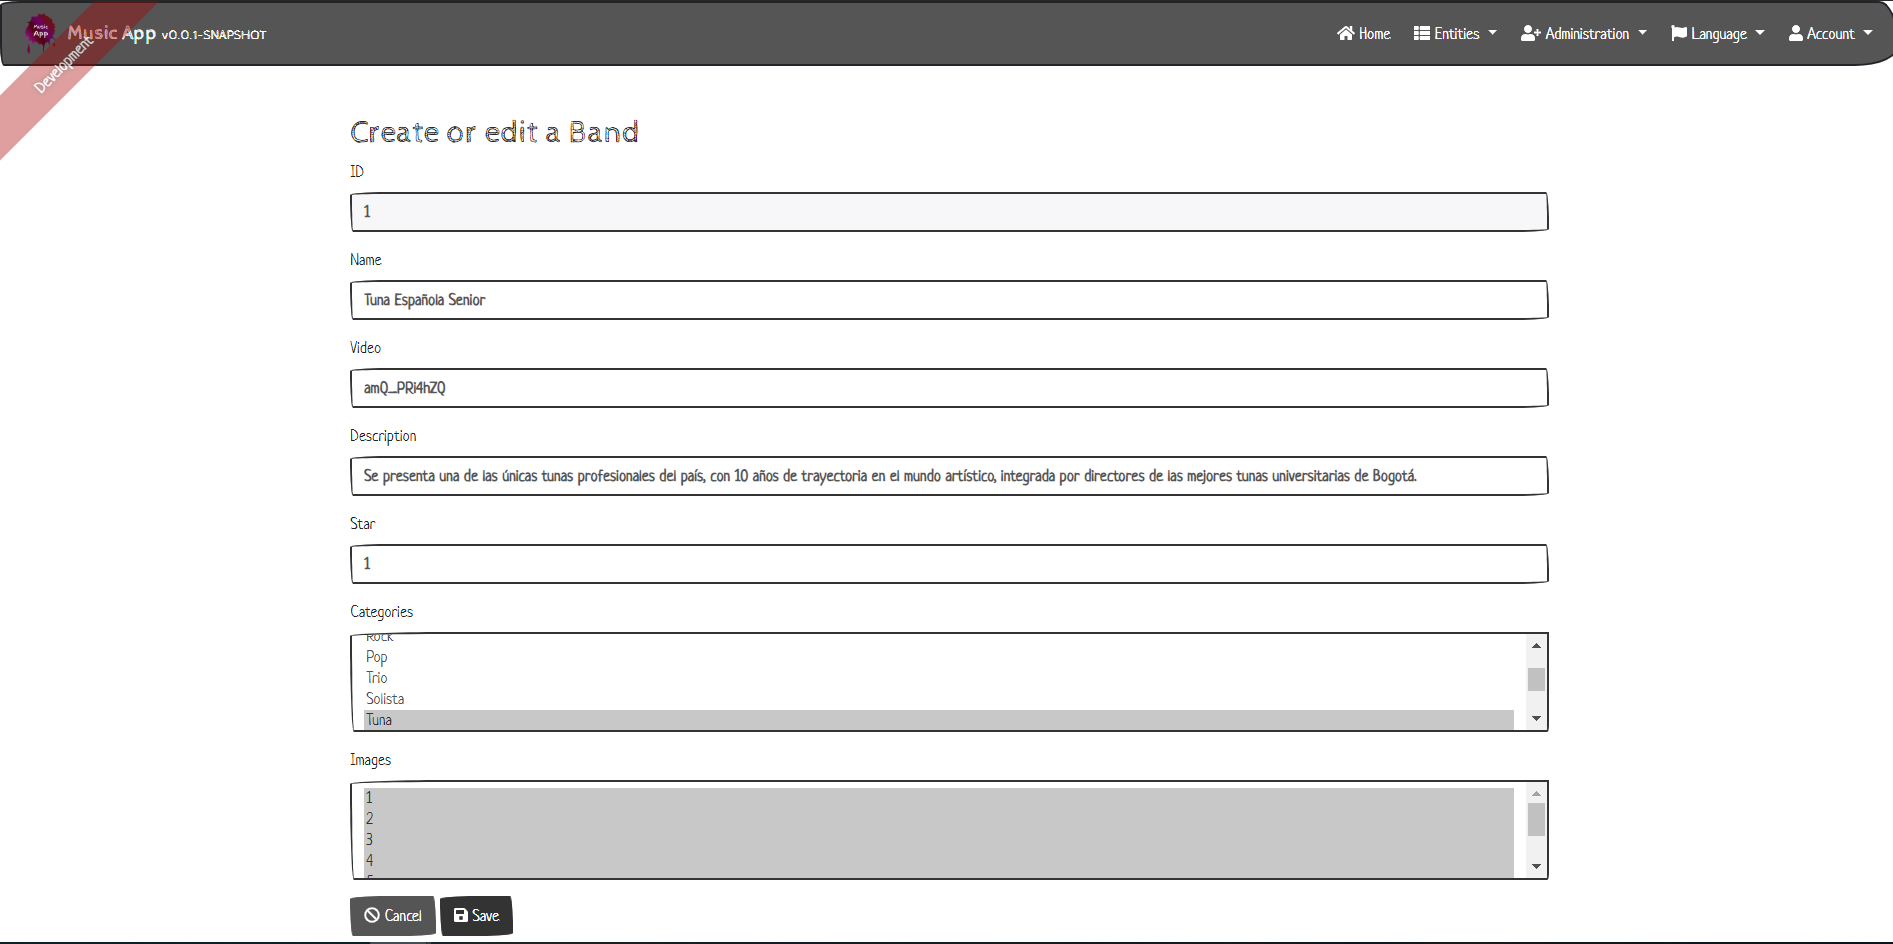
\includegraphics[width=\linewidth]{Desarrollo/Interfaces/Interfaces/imgs/BandEdit.PNG}
\caption{Editar o crear grupos musicales}
\end{figure}

\newpage

\subsubsection{Listar las url de las imágenes registradas en el sistema}
En esta vista podemos ver las url de las imágenes registradas en el sistema.
\begin{figure}[h!]
 \centering
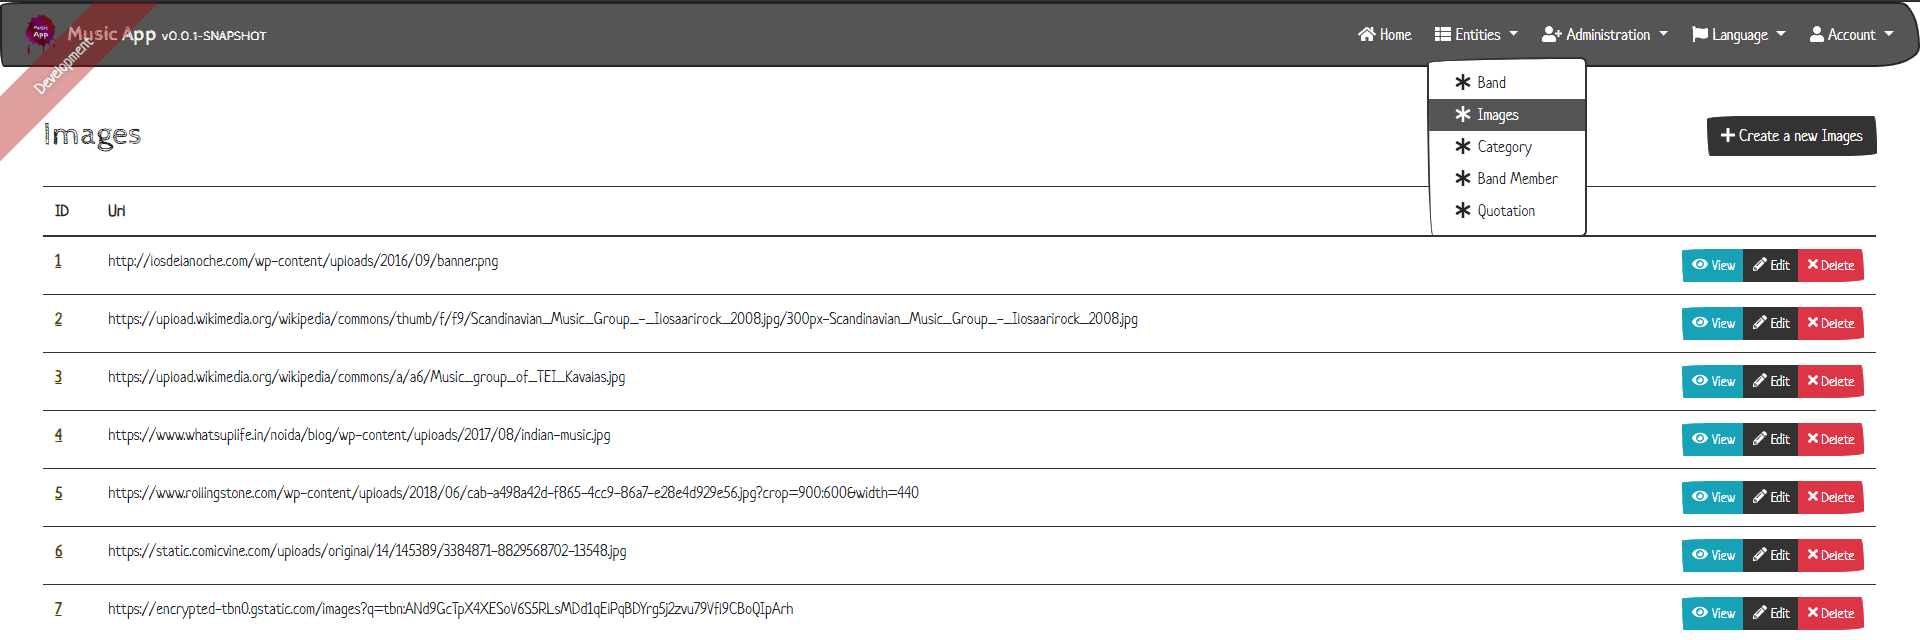
\includegraphics[width=\linewidth]{Desarrollo/Interfaces/Interfaces/imgs/ImagesList.PNG}
\caption{Lista de url de imágenes}
\end{figure}



\subsubsection{Editar o crear las url de las imágenes registradas en el sistema}
En esta vista podemos editar las url de las imágenes registradas en el sistema.
\begin{figure}[h!]
 \centering
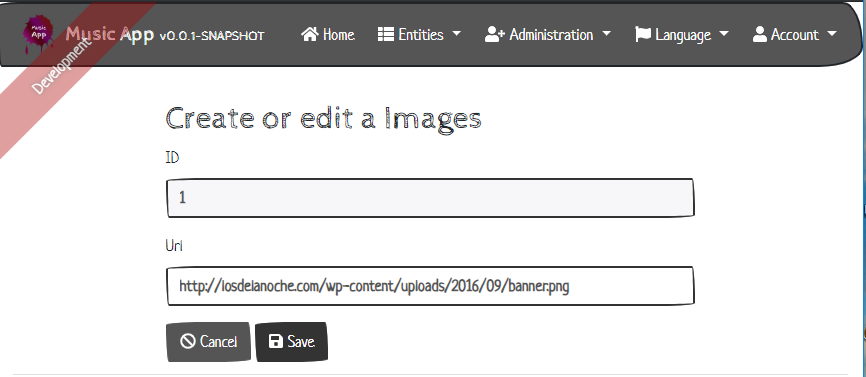
\includegraphics[width=0.8\linewidth]{Desarrollo/Interfaces/Interfaces/imgs/ImagesEdit.PNG}
\caption{Editar o crear url de imagen}
\end{figure}

\newpage

\subsubsection{Listar categorías}
En esta vista podemos ver y organizar el nombre de todas las categorías.
\begin{figure}[h!]
 \centering
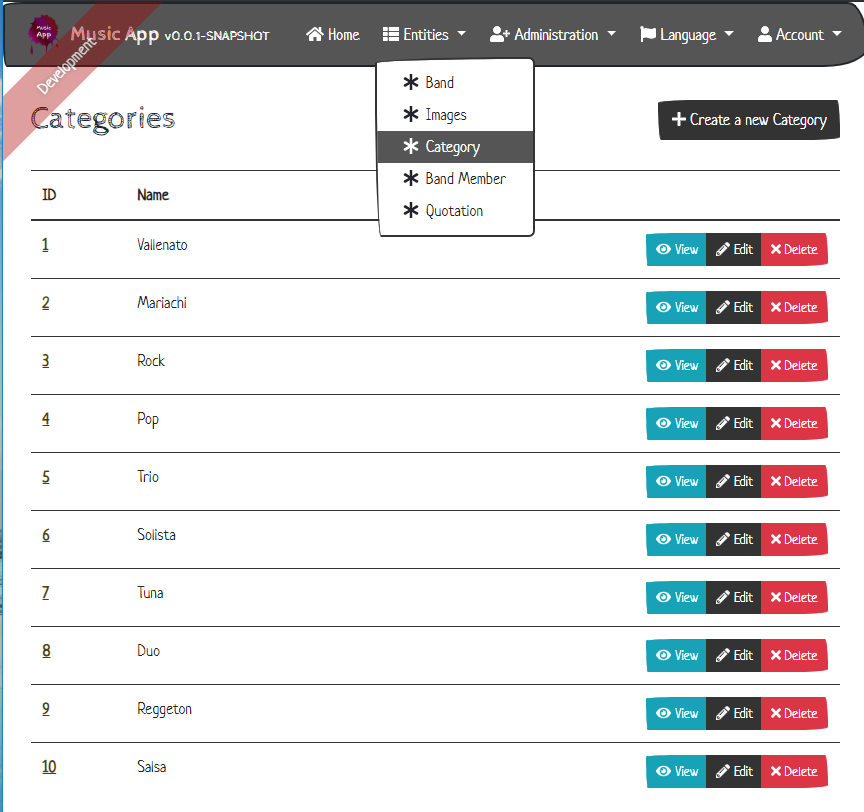
\includegraphics[width=\linewidth]{Desarrollo/Interfaces/Interfaces/imgs/categoryList.PNG}
\caption{Lista categorías}
\end{figure}

\newpage

\subsubsection{Editar o crear categorías}
En esta vista podemos editar las categorías de los grupos musicales.
\begin{figure}[h!]
 \centering
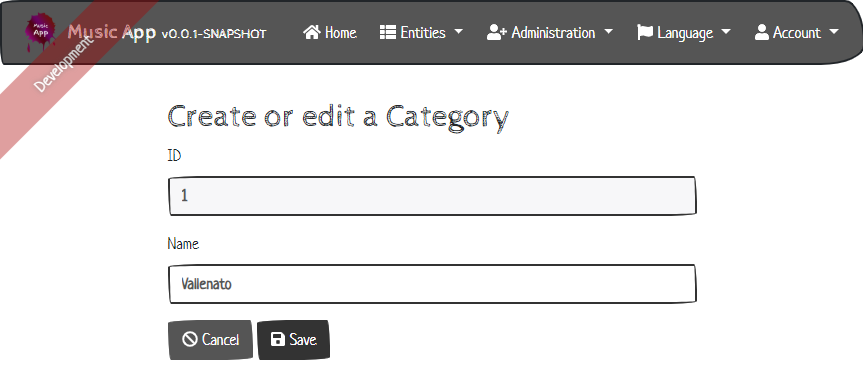
\includegraphics[width=0.8\linewidth]{Desarrollo/Interfaces/Interfaces/imgs/categoryEdit.PNG}
\caption{Editar o crear categorías}
\end{figure}

\subsubsection{Usuarios asociados a los grupos musicales}
En esta vista podemos ver y organizar los usuarios que están asociados a los grupos musicales, es decir, se pueden asociar todos los integrantes del grupo, que cada uno tenga su propio login pero pueden ver la misma información de su grupo musical.
\begin{figure}[h!]
 \centering
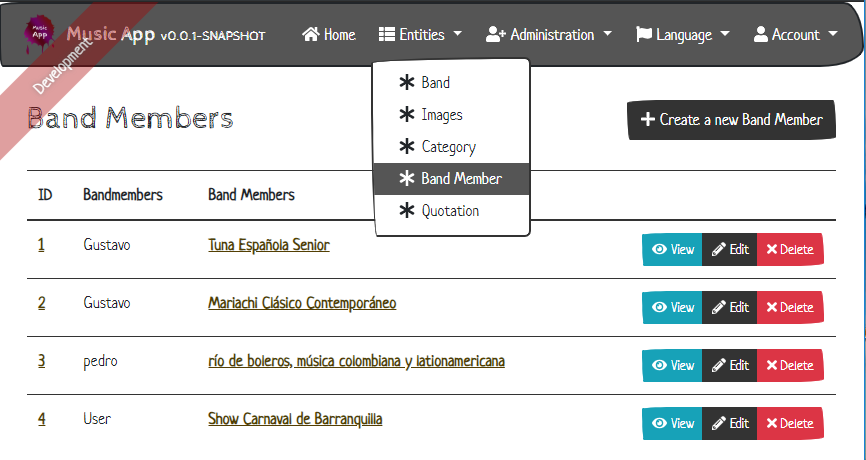
\includegraphics[width=\linewidth]{Desarrollo/Interfaces/Interfaces/imgs/BandMemberList.PNG}
\caption{Lista músicos asociados al grupo musical}
\end{figure}

\newpage

\subsubsection{Editar o crear usuarios asociados a los grupos musicales}
En esta vista podemos editar el músico asociado con algún grupo musical.
\begin{figure}[h!]
 \centering
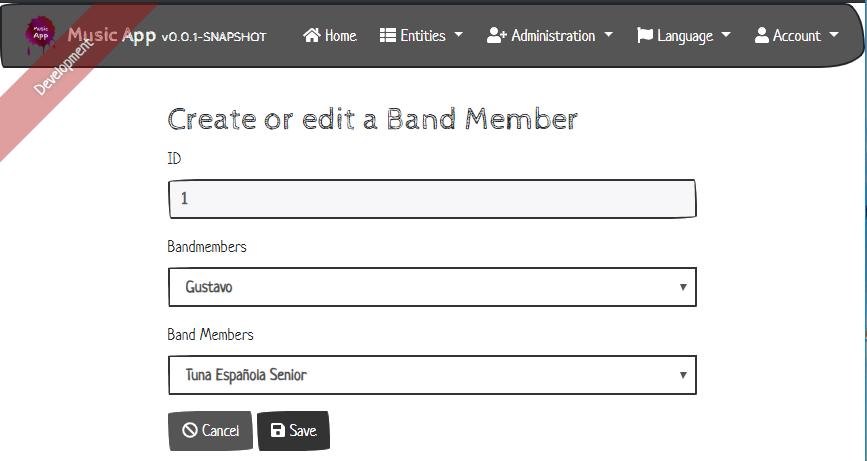
\includegraphics[width=0.8\linewidth]{Desarrollo/Interfaces/Interfaces/imgs/BandMemberEdit.PNG}
\caption{Editar o crear músicos asociados al grupo musical}
\end{figure}

\subsubsection{Usuarios}
En esta vista podemos ver y organizar los usuarios registrados en el sistema con la información básica y sus roles
\begin{figure}[h!]
 \centering
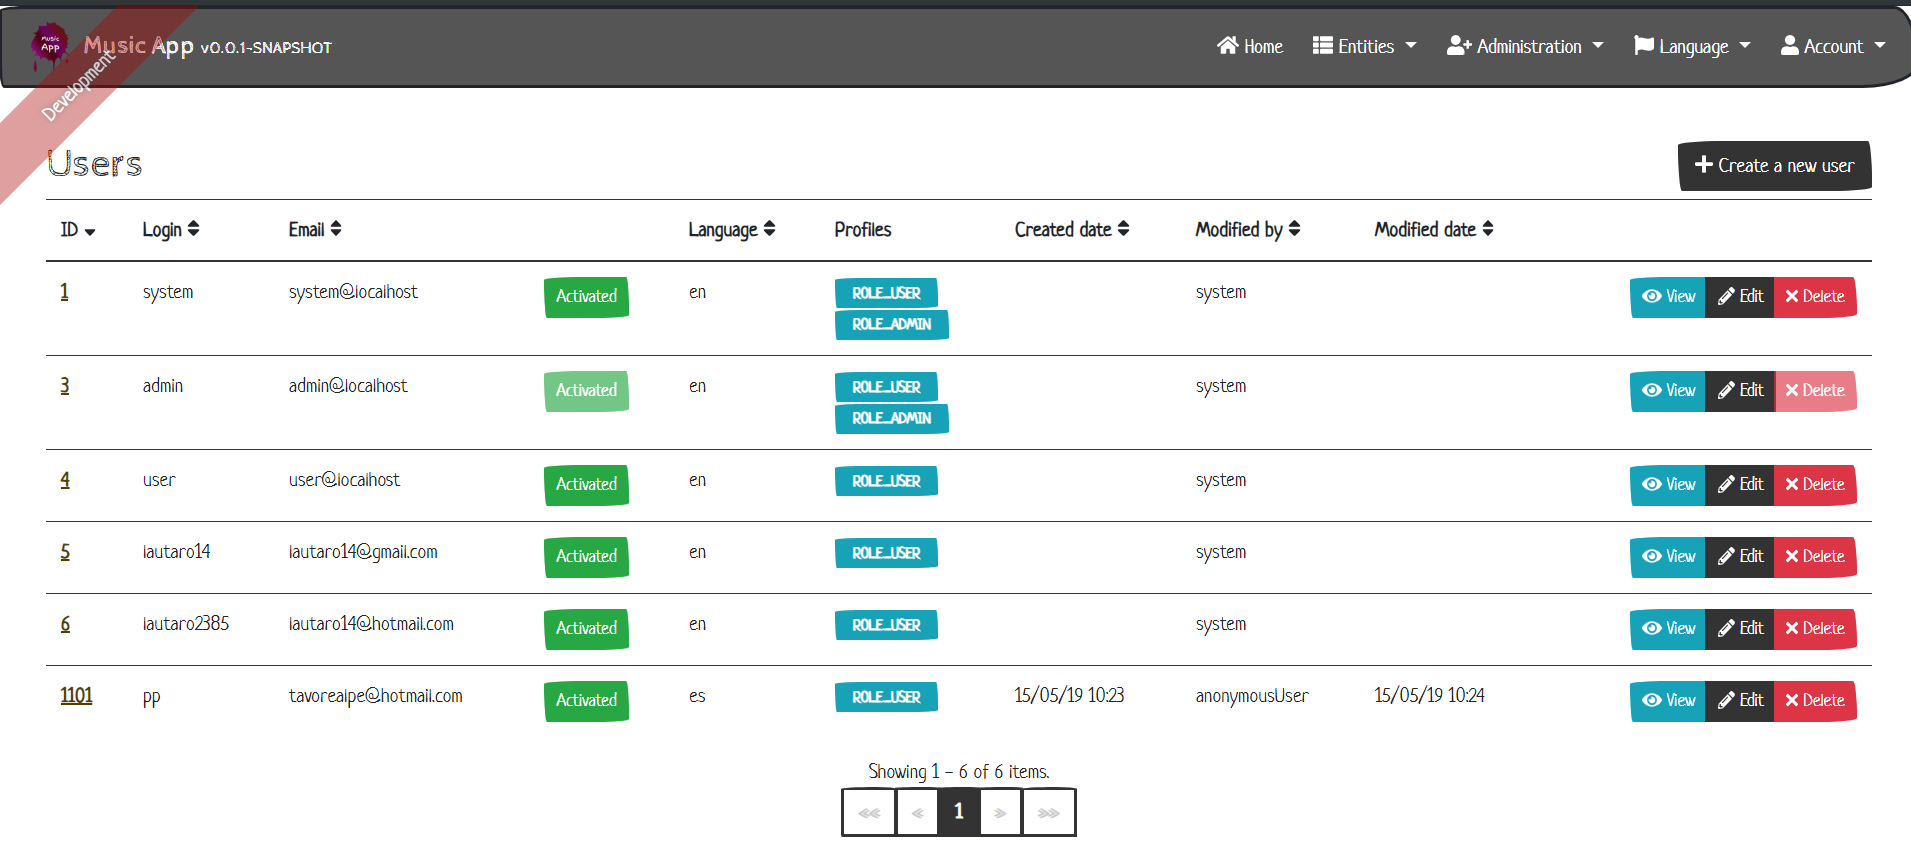
\includegraphics[width=\linewidth]{Desarrollo/Interfaces/Interfaces/imgs/UserList.PNG}
\caption{Lista usuarios}
\end{figure}

\newpage

\subsubsection{Editar o crear usuarios}
En esta vista podemos editar el músico asociado con algún grupo musical.
\begin{figure}[h!]
 \centering
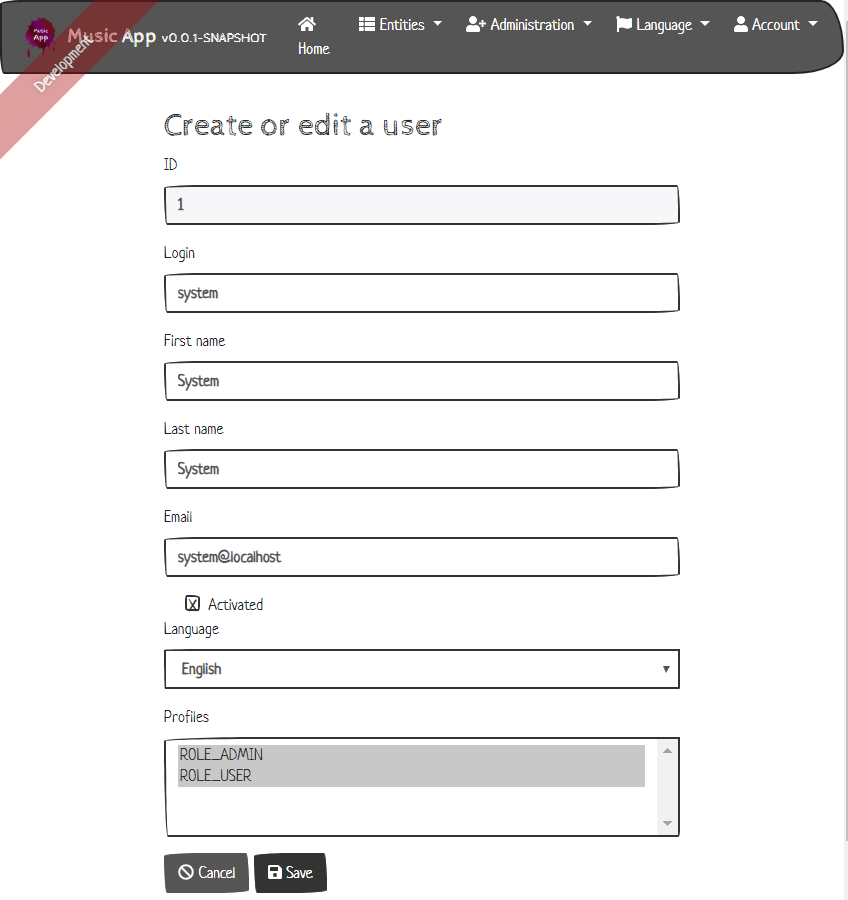
\includegraphics[width=0.8\linewidth]{Desarrollo/Interfaces/Interfaces/imgs/UserEdit.PNG}
\caption{Editar o crear usuarios}
\end{figure}

\newpage